\documentclass[border=6pt]{standalone}
\usepackage{tikz}
\usetikzlibrary{arrows.meta,positioning}
\begin{document}
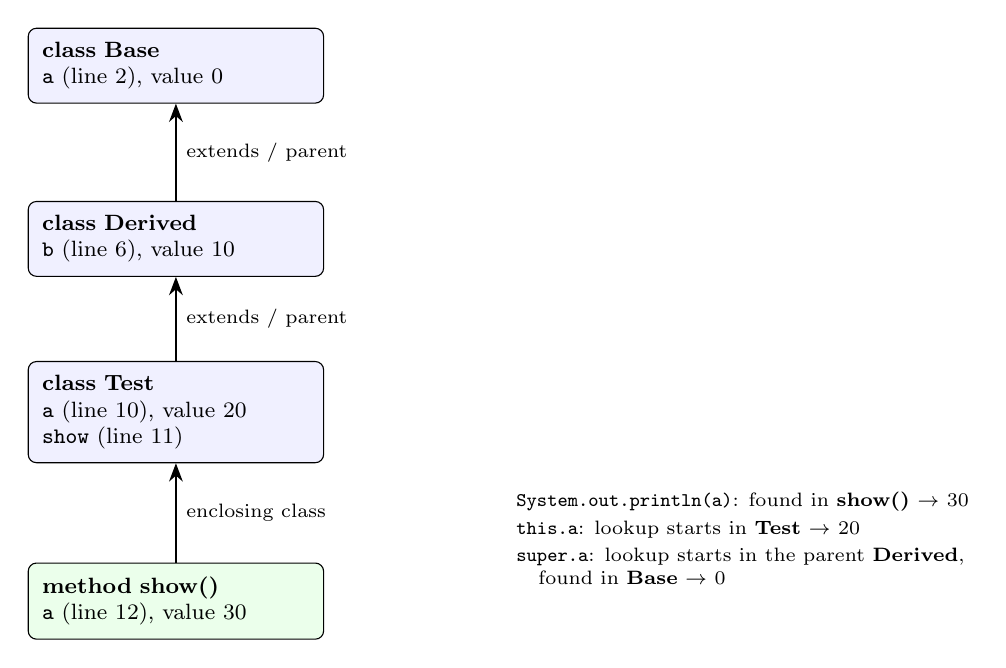
\begin{tikzpicture}[>=Stealth,font=\small,
  tbl/.style={draw,rounded corners=3pt,fill=blue!6,align=left,inner sep=5pt,font=\footnotesize,text width=3.4cm}]
\node[tbl] (B) at (0,0) {\textbf{class Base}\\ \texttt{a}\ (line 2), value 0};
\node[tbl] (D) at (0,-2.2) {\textbf{class Derived}\\ \texttt{b}\ (line 6), value 10};
\node[tbl] (T) at (0,-4.4) {\textbf{class Test}\\ \texttt{a}\ (line 10), value 20\\ \texttt{show}\ (line 11)};
\node[tbl,fill=green!8] (S) at (0,-6.8) {\textbf{method show()}\\ \texttt{a}\ (line 12), value 30};
\draw[->,thick] (D) -- node[right,font=\scriptsize]{extends / parent} (B);
\draw[->,thick] (T) -- node[right,font=\scriptsize]{extends / parent} (D);
\draw[->,thick] (S) -- node[right,font=\scriptsize]{enclosing class} (T);
\node[font=\scriptsize,align=left,anchor=west] at (4.2,-6.0) {\texttt{System.out.println(a)}: found in \textbf{show()} $\to$ 30\\[2pt] \texttt{this.a}: lookup starts in \textbf{Test} $\to$ 20\\[2pt] \texttt{super.a}: lookup starts in the parent \textbf{Derived},\\ \hspace*{1em}found in \textbf{Base} $\to$ 0};
\end{tikzpicture}
\end{document}
